\section{Estimating road speeds}
\label{sec:vehicle_speeds}

Now that we have estimated the necessary vehicle states and their respective trajectories, we are able to infer a vehicle's \emph{average speed} along the $\ell^\text{th}$ road segment, $\Vtt_{\ell}$. These estimates are used later to update the \emph{road network state} (\cref{cha:network_model}) and ultimately estimate arrival times (\cref{cha:prediction}).


Estimation of average road speed is perfomed by first computing the \emph{travel time} along each road segment as the bus traverses the network. To do so, we record the time when the vehicle starts and ends each segment, $\Vsegstart_\ell$ and $\Vsegend_\ell$, respectively, and simply take the difference to obtain the travel time in seconds. By using a particle filter, we simply record these values for each particle as it is transitioned to each new state. Finally, transforming to average speed uses the length of the segment, $\Tseglen_\ell$, in meters, and the standard speed formula (speed = distance / time):
\begin{equation}
\label{eq:vehicle_avg_speed}
\Vtt_\ell = \frac{\Tseglen_\ell}{\Vsegend_\ell - \Vsegstart_\ell}.
\end{equation}


Since estimating \cref{eq:vehicle_avg_speed} is straighforward for each individual particle, the posterior distribution of the vehicle's average travel time along segment $\ell$, given all observations up to and including time $\Vtime_k$, is again approximated using the Dirac measure,
\begin{equation}
\label{eq:pf_speed_dist}
p(\Vtt_\ell | \Vobs_{1:k}) \approx
\sum_{i=1}^\Np \Pwt_k \dirac(\Vtt_\ell - \Vtt\vi_\ell).
\end{equation}
In situations where only some of the particles have completed travel along a segment, we wait until the next iteration to re-check that all particles have completed it and, since start and end times are stored for each individual particle, we can still estimate average speed.



In order to explore the accuracy of the models presented in \cref{sec:vehicle_model}, a simple vehicle simulation was performed with known road speeds and involved tracking the vehicle along the route while ignoring bus stops. In a second simulation, the bus stopped at each stop, and the particle filter implemented the bus stop behaviour model. For each, we used three different sampling methods:
\begin{itemize}
\item uniform sampling with 10~second intervals;
\item uniform sampling with 30~second intervals; and
\item non-uniform sampling at nodes.
\end{itemize}
As mentioned in \cref{sec:vp_data}, the last of these is, in fact, a common feature of the Auckland Transport data; we discuss the complications further in \cref{sec:pf_implementation}. In each simulation, we implemented the three variations of the transition function: $\Vtrans_{A1}$, $\Vtrans_{A2}$, and $\Vtrans_{A3}$.



The posterior mean travel time was used
to examine the estimation accuracy of the models and compare them,
which is simple to calculate from the particle filter estimates of travel time by
the weighted mean of the sample,
\begin{equation}
\label{eq:pf_travel_time_mean}
\bar\Vtt_\ell =
\E{\Vtt_\ell | \Vobs_{1:k}} =
\sum_{i=1}^\Np \Pwt_k \Vtt\vi_\ell
\end{equation}


To evaluate and compare the estimation performance of the models, we use \gls{rmse} and \gls{mae}, which are defined in \cref{app:error-functions}.


\subsubsection{Simulation A: general vehicle model}
\label{sec:vehicle_sim_A}





The simulated data, shown in \cref{fig:sim1_graph1}, uses the transition model described by $\Vtrans_{A1}$ to simulate a vehicle trajectory, and uses several time point sampling methods: uniform sampling with high (\cref{fig:sim1_graph2}) and low (\cref{fig:sim1_graph3}) frequency, and non-uniform sampling (\cref{fig:sim1_graph4}), which is more in line with how the Auckland Transport data is collected.


The goal of the simulation is to estimate the average vehicle speeds along several road segments, as well as the associated uncertainty. The simulation was performed in R \citep{rcore} using $\Np = 2000$ particles per vehicle, and so the implementation is slightly different from the C++ one defined in \cref{sec:pf_implementation}.

\begin{knitrout}\small
\definecolor{shadecolor}{rgb}{0.969, 0.969, 0.969}\color{fgcolor}\begin{figure}
\subfloat[The simulated data.\label{fig:sim1_graph1}]{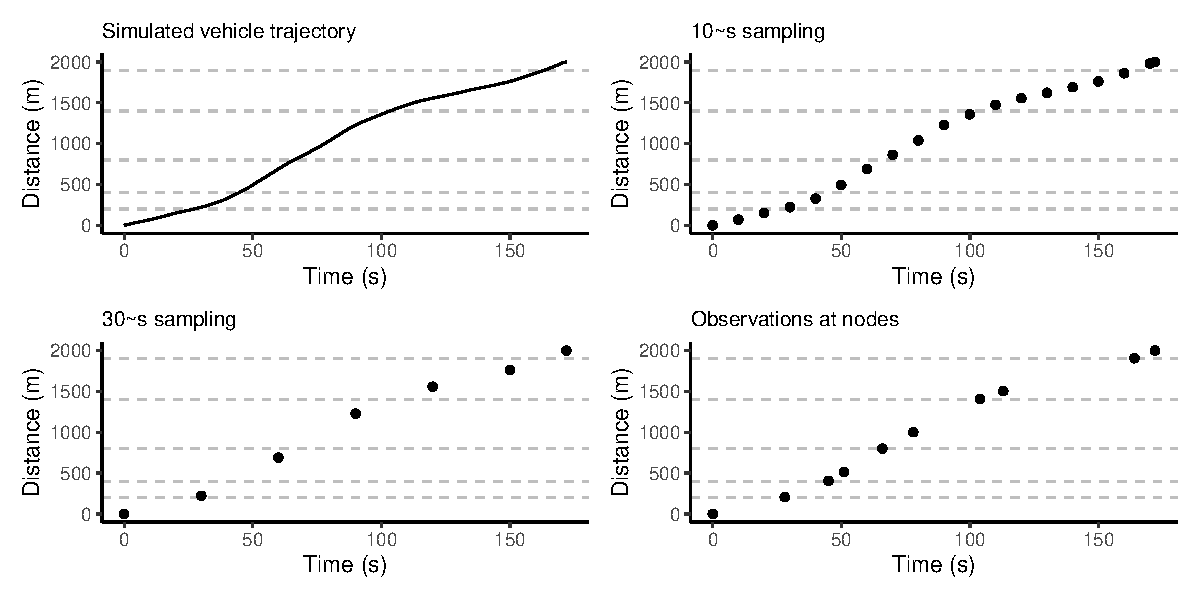
\includegraphics[width=.49\linewidth]{figure/sim1_graph-1} }
\subfloat[10~s sampling.\label{fig:sim1_graph2}]{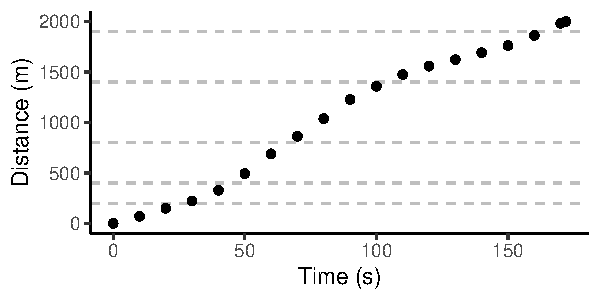
\includegraphics[width=.49\linewidth]{figure/sim1_graph-2} }\newline
\subfloat[30~s sampling.\label{fig:sim1_graph3}]{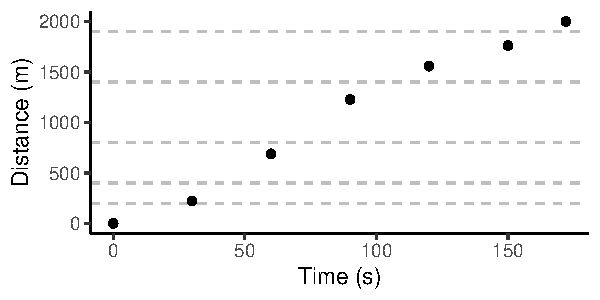
\includegraphics[width=.49\linewidth]{figure/sim1_graph-3} }
\subfloat[Observations at bus stops and intersections.\label{fig:sim1_graph4}]{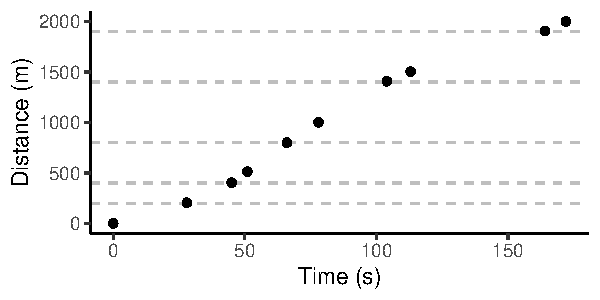
\includegraphics[width=.49\linewidth]{figure/sim1_graph-4} }\caption[Simulated vehicle trajectory, with five road segments]{Simulated vehicle trajectory, with five road segments.}\label{fig:sim1_graph}
\end{figure}


\end{knitrout}

\begin{knitrout}\small
\definecolor{shadecolor}{rgb}{0.969, 0.969, 0.969}\color{fgcolor}\begin{figure}
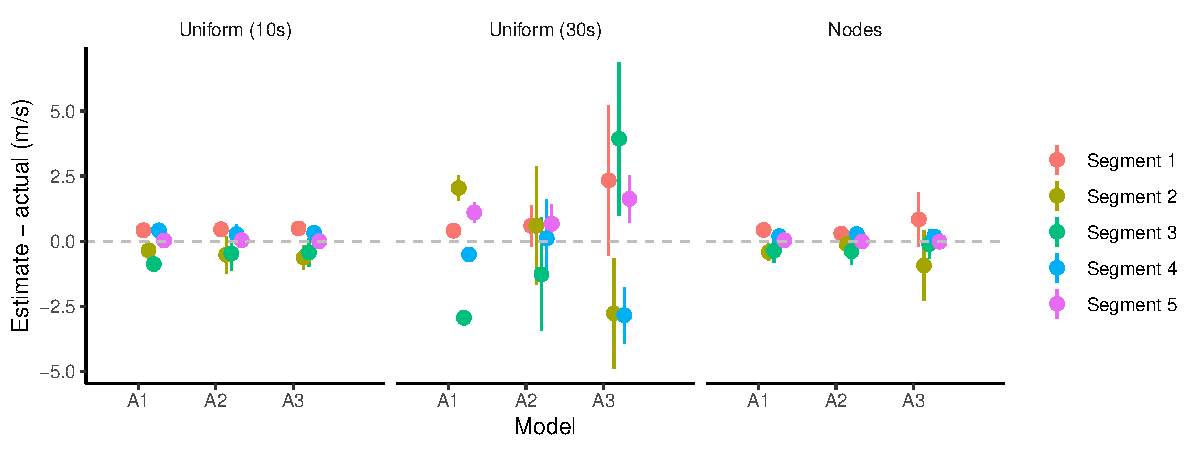
\includegraphics[width=\linewidth]{figure/sim1_pf-1} \caption[Simulation results for the three models (rows) applied to the data from three sampling methods (columns), using $\Np=2000$ particles]{Simulation results for the three models (rows) applied to the data from three sampling methods (columns), using $\Np=2000$ particles. The standard deviation of the particle travel times is represented as error bars, though in many cases the error is too small to display.}\label{fig:sim1_pf}
\end{figure}


\end{knitrout}

\begin{knitrout}\small
\definecolor{shadecolor}{rgb}{0.969, 0.969, 0.969}\color{fgcolor}\begin{figure}
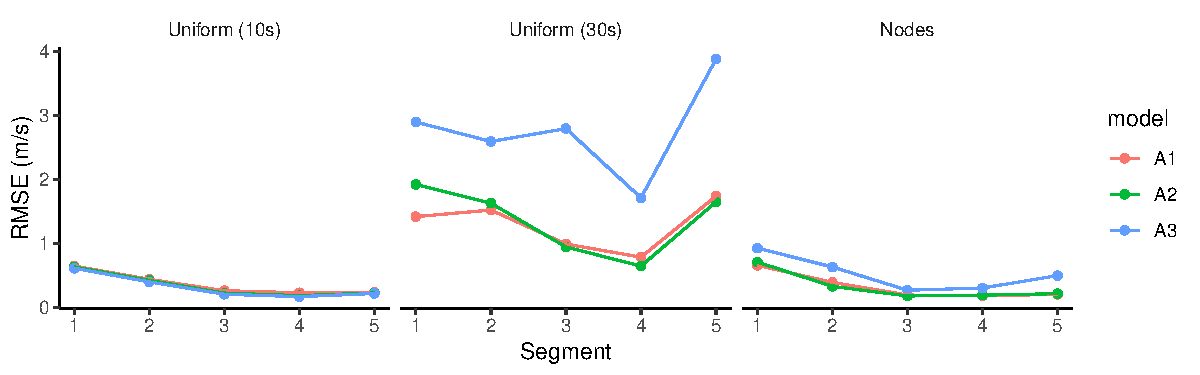
\includegraphics[width=\maxwidth]{figure/sim1_pf_full-1} \caption[Speed estimation results for 100 simulations]{Speed estimation results for 100 simulations. In each the vehicle trajectory is simulated using a different seed, and the speed estimate is taken as the mean of the particle speeds along each segment.}\label{fig:sim1_pf_full}
\end{figure}

\begin{table}

\caption{\label{tab:sim1_pf_full}RMSE of average speed estimation}
\centering
\fontsize{8}{10}\selectfont
\begin{tabular}[t]{llrr}
\toprule
Sampling method & Model & RMSE (m/s) & MAE (m/s)\\
\midrule
Uniform (10s) & A1 & 0.40 & 0.27\\
 & A2 & 0.38 & 0.26\\
 & A3 & 0.36 & 0.24\\
\midrule
Uniform (30s) & A1 & 1.34 & 0.95\\
 & A2 & 1.44 & 1.01\\
 & A3 & 2.87 & 2.07\\
\midrule
Nodes & A1 & 0.38 & 0.25\\
 & A2 & 0.38 & 0.25\\
 & A3 & 0.58 & 0.36\\
\bottomrule
\end{tabular}
\end{table}


\end{knitrout}

The results of the simulation applied to the data displayed in \cref{fig:sim1_graph} is shown in \cref{fig:sim1_pf}. Under the high-frequency uniform sampling method, all models perform similarly with high precision (the errors are all close to zero) and accuracy (the uncertainty is small enough that it does not show up). For the low-frequency sampling, however, model A3 shows slightly better precision than A1 and A2. Finally, for sampling at nodes, the models all perform similarly except in their estimation of speed for segment 5, which A1 and A2 estimate with high uncertainty.


To further examine the comparative performance of the models, we repeated the simulation 100~times using the same segments and sampling points, but varying the underlying trajectory of the vehicle. From the results displayed in \cref{fig:sim1_pf_full}, the most obvious feature is the difficulty estimating the last segment: this would likely be improved by including a likelihood on arrival time (since, as it stands, the particles may arrive very early for the last stop and, since this is the end of the route, they stay there until the observation). Model A2 appears to estimate with higher precision than either of the others, particularly for the final segment. A1 has better accuracy, overall.



\subsubsection{Simulation B: bus stop model}
\label{sec:vehicle_sim_B}

In the previous simulation, we assumed the vehicle travelled along the route without stopping. Now, we add bus stopping behaviour to the model, as shown in \cref{fig:sim2_graph}. In the simulated data, the bus stops at all stops with an unknown dwell time, and we use $\pi=0.5$ for the stopping probability in the particle filter when estimating vehicle state. The sampling is the same as before: 10~second and 30~second rates, as well as observations at nodes (intersections and bus stops).






\begin{knitrout}\small
\definecolor{shadecolor}{rgb}{0.969, 0.969, 0.969}\color{fgcolor}\begin{figure}
\subfloat[The simulated data.\label{fig:sim2_graph1}]{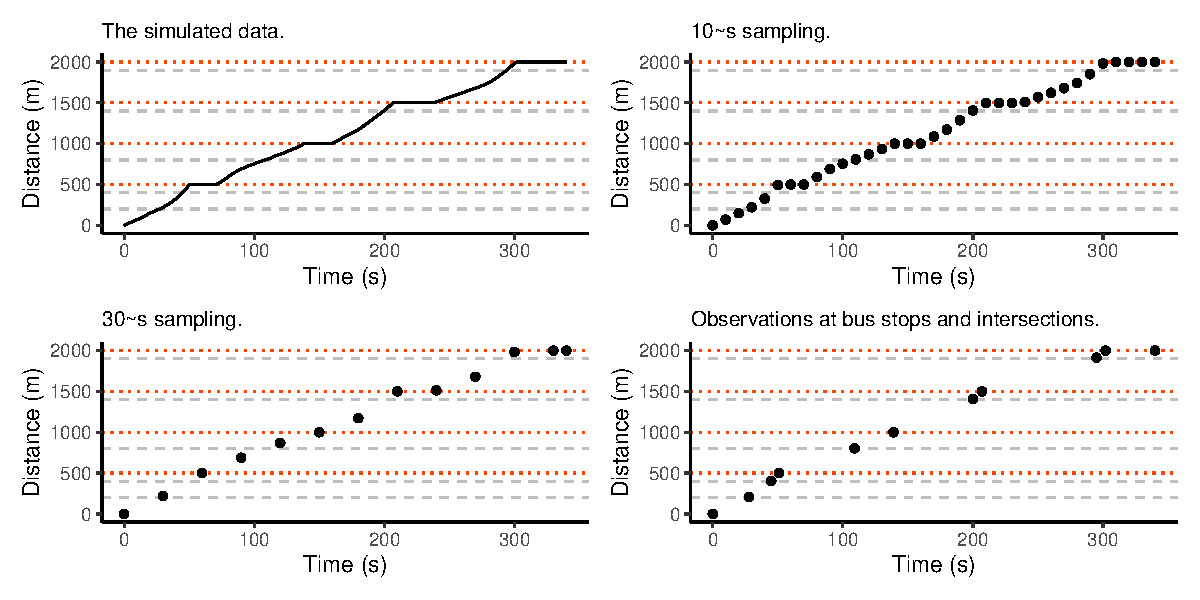
\includegraphics[width=.49\linewidth]{figure/sim2_graph-1} }
\subfloat[10~s sampling.\label{fig:sim2_graph2}]{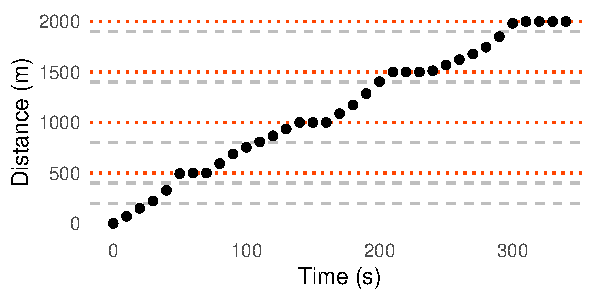
\includegraphics[width=.49\linewidth]{figure/sim2_graph-2} }\newline
\subfloat[30~s sampling.\label{fig:sim2_graph3}]{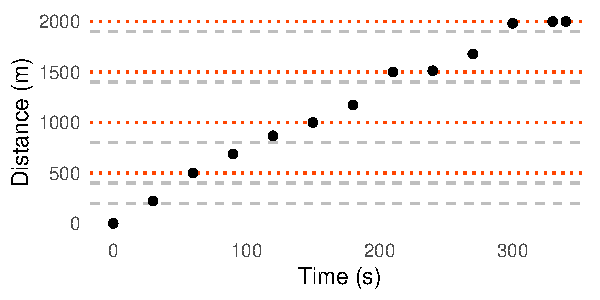
\includegraphics[width=.49\linewidth]{figure/sim2_graph-3} }
\subfloat[Observations at bus stops and intersections.\label{fig:sim2_graph4}]{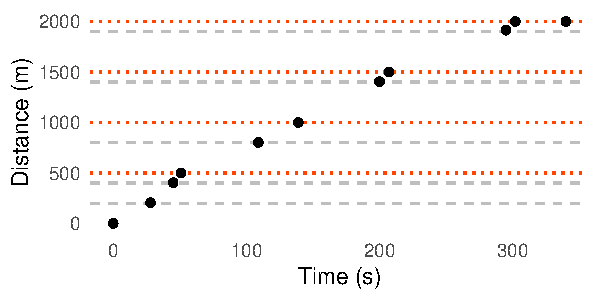
\includegraphics[width=.49\linewidth]{figure/sim2_graph-4} }\caption[Simulated vehicle trajectory, with five road segments and three intermediate stops]{Simulated vehicle trajectory, with five road segments and three intermediate stops.}\label{fig:sim2_graph}
\end{figure}


\end{knitrout}


The results of the simulation are shown in \cref{fig:sim2_pf}, where we see somewhat similar results to before: the models perform similarly well under high-frequency uniform sampling, with lower precision under low-frequency sampling. For sampling at nodes, again we see the same issue with estimation of speed for the final segment, but otherwise the models perform similarly.

\begin{knitrout}\small
\definecolor{shadecolor}{rgb}{0.969, 0.969, 0.969}\color{fgcolor}\begin{figure}
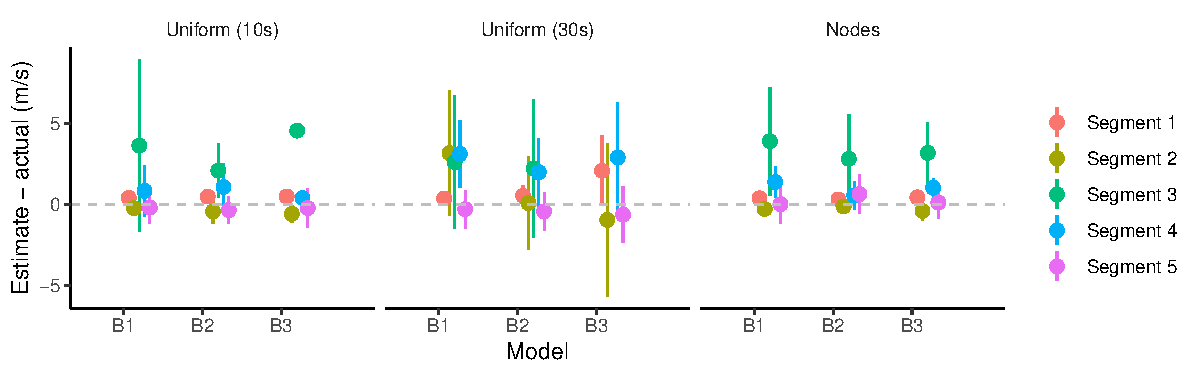
\includegraphics[width=\linewidth]{figure/sim2_pf-1} \caption[Simulation results for the three models (rows) applied to the data from three sampling methods (columns), using $\Np=2000$ particles]{Simulation results for the three models (rows) applied to the data from three sampling methods (columns), using $\Np=2000$ particles. [details].}\label{fig:sim2_pf}
\end{figure}


\end{knitrout}


Repeating the simulation 100~times with different vehicle trajectories, we can better compare the models (\cref{fig:sim2_pf_full}, which excludes the final segment). Uncertainties are now much higher, particularly under low-frequency sampling. Models A1 and A2 appear to perform similarly, and better estimate speed along slower segments, versus A3 which shows has difficulty even with slow segments.

\begin{knitrout}\small
\definecolor{shadecolor}{rgb}{0.969, 0.969, 0.969}\color{fgcolor}\begin{figure}
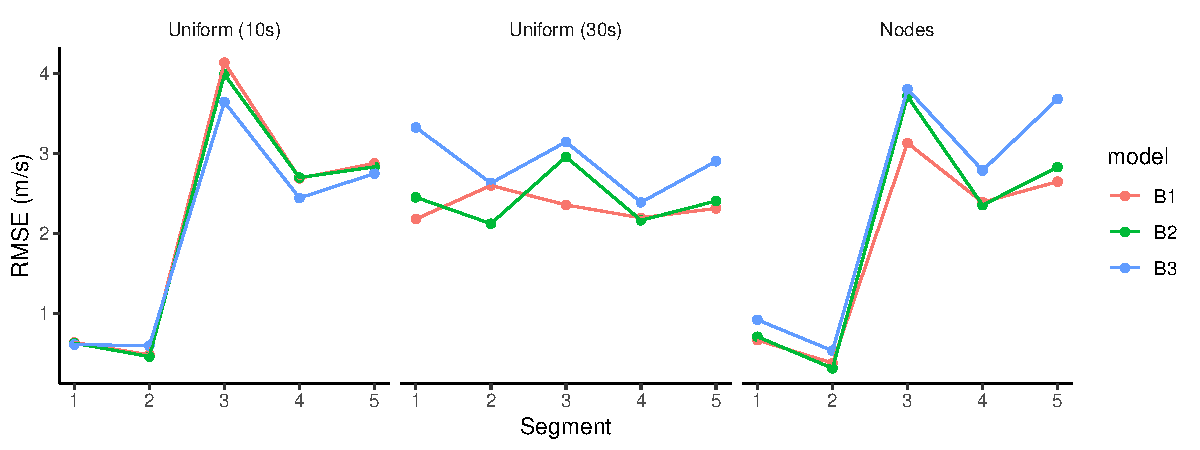
\includegraphics[width=\maxwidth]{figure/sim2_pf_full-1} \caption[Speed estimation results for 100 simulations]{Speed estimation results for 100 simulations. In each the vehicle trajectory is simulated using a different seed, and the speed estimate is taken as the mean of the particle speeds along each segment.}\label{fig:sim2_pf_full}
\end{figure}

\begin{table}

\caption{\label{tab:sim2_pf_full}RMSE of average speed estimation}
\centering
\fontsize{8}{10}\selectfont
\begin{tabular}[t]{llrr}
\toprule
Sampling method & Model & RMSE (m/s) & MAE (m/s)\\
\midrule
Uniform (10s) & A1 & 2.56 & 1.40\\
 & A2 & 2.51 & 1.35\\
 & A3 & 2.34 & 1.35\\
\midrule
Uniform (30s) & A1 & 2.34 & 1.58\\
 & A2 & 2.43 & 1.63\\
 & A3 & 2.90 & 2.14\\
\midrule
Nodes & A1 & 2.15 & 1.31\\
 & A2 & 2.36 & 1.35\\
 & A3 & 2.70 & 1.57\\
\bottomrule
\end{tabular}
\end{table}


\end{knitrout}



Comparing the estimates numerically using \gls{rmse} (\cref{tab:sim2_pf_full}) we see, within each sampling method, the errors are similar. Models A1 and A2 perform very similarly, while model A3 is consistently higher.



\subsubsection{Simulation C: bus stops as nodes with unknown intersections}
\label{sec:vehicle_sim_C}

This time, we perform a simulation that more closely replicates the Auckland Transport system we are modelling. In it, we no longer know the locations of intersections, so road segments are specified between stops instead. In this simulation, the bus may still stop at intersections, but the underlying model does not know where these are. The goal is to esimate travel time along segments (which is now the \emph{link time} between stops).
